\chapter{Interrogazione del data mart}
In questa sezione vengono definite le interrogazioni sui datamart che sono state effettuate.

Tutte le richieste fatte ai datamart vengono, di conseguenza, effettuate attraverso interroga-
zioni ad un DBMS Mysql.

\section{Visualizzazione settimanale}

\begin{figure}[H]                                                                                                                                                            
\centering                                                                                                                                                                   
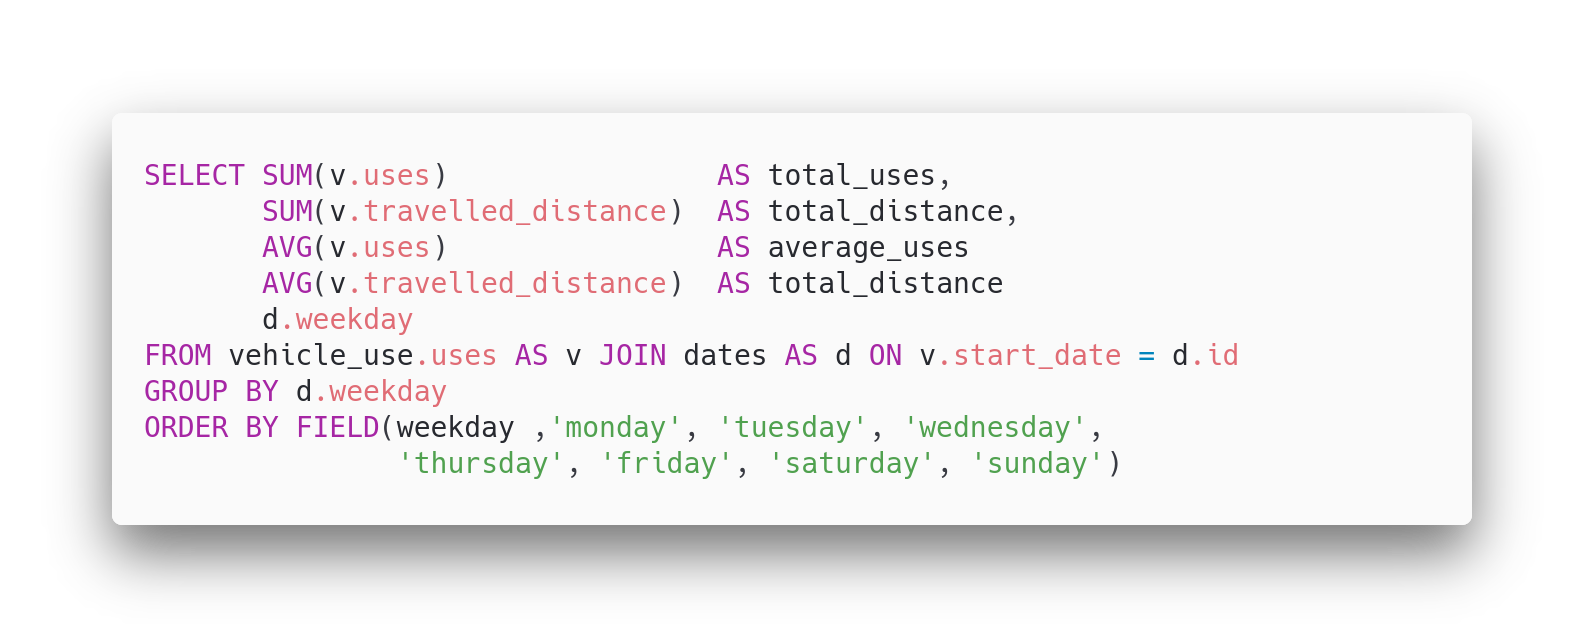
\includegraphics[width=\textwidth]{images/query1}                                                                                                                                   
\label{fig:query1}                                                                                                                                                           
\end{figure}

\iffalse
SELECT SUM(v.uses)                AS total_uses, 
	   SUM(v.travelled_distance)  AS total_distance, 
       AVG(v.uses)                AS average_uses
       AVG(v.travelled_distance)  AS total_distance
       d.weekday
FROM vehicle_use.uses AS v JOIN dates AS d ON v.start_date = d.id
GROUP BY d.weekday
ORDER BY FIELD(weekday ,'monday', 'tuesday', 'wednesday',
			   'thursday', 'friday', 'saturday', 'sunday')
\fi


\section{Analisi sui numeri di utilizzi in presenza di sciopero}
